A honeycomb grows in layers around a single central hexagonal cell. Layer $1$ is the central cell itself; layer $2$ is the ring of $6$ cells surrounding it, then layer $3$ adds the next ring, and so on --- the comb with $n$ layers contains the central cell plus rings $2, 3, \ldots, n$.

The picture shows the honeycomb with $3$ layers: the central cell, then rings of $6$ and $12$ cells --- $19$ cells in total.

\begin{center}
  \def \htmlPixelsInCm {45}
  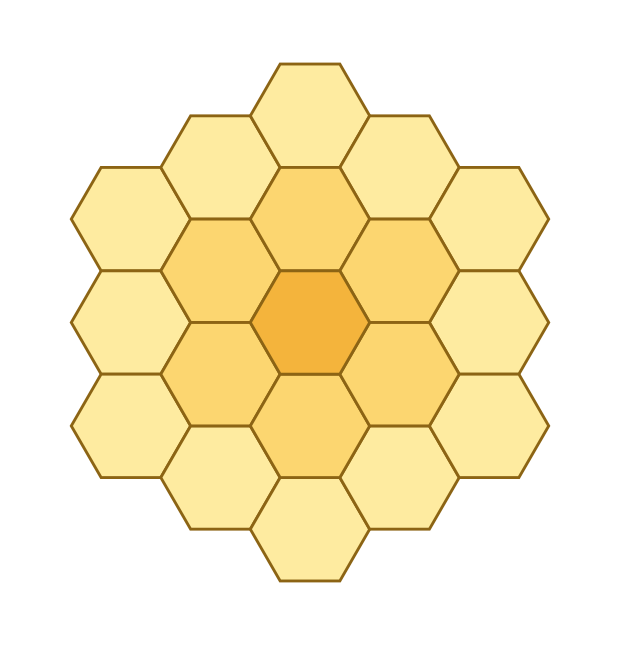
\includegraphics[width=6.5cm]{honeycomb.svg} \\[4pt]
  \small{A honeycomb with $3$ layers and $19$ hexagonal cells.}
\end{center}

Count the total number of hexagonal cells in a honeycomb with $n$ layers.
